\documentclass{book}  
\usepackage{amsmath,lmodern} 
\usepackage{fancyhdr}
\usepackage{fontspec}
\usepackage[UTF8]{ctex}
\usepackage{ragged2e}
\usepackage{graphicx}
\usepackage{float}
\usepackage{listings}
\usepackage{subfigure}

\setmainfont{Times New Roman}
\renewcommand\tablename{Table}

\begin{document}
\zihao{4}
\centering
节选第五章 \\

\hspace*{\fill} \\
\zihao{5}
\justifying
\noindent
5.3. Use the inverse transform method to generate a random variable having distribution function
$$
  F(x) = \frac{x^{2}+x}{2}, \ \ \  0\leq x\leq 1
$$
\noindent
翻译:使用逆变换方法生成具有如上分布函数的随机变量 \\
解:令$y=\frac{x^{2}+x}{2}$,则$x=\sqrt{\frac{1}{4}+2y}-\frac{1}{2}$, 模拟生成$x$即可,代码如下
\lstset{language = R}
\begin{lstlisting}
    library(ggplot2)
    n <- 188888
    U <- runif(n)
    X <- sqrt(0.25+2*U)-0.5
    #绘制分布函数图像
    dataResult <- data.frame(data = X)
    p <- ggplot(dataResult, aes(x = data)) 
    p + stat_ecdf(size = 0.1) + 
        labs(title = "X的分布函数图像",
             x = "X",
             y = "累积概率") + 
        theme(plot.title = element_text(
            color = "blue", face = "bold", hjust = 0.5
            ))
    #绘制概率密度图
    hist(X, freq = FALSE, breaks = 100, 
         col = "yellow", main = "X的密度函数图像")
    #拟合理论密度曲线
    Y <- seq(0,1,0.001)
    lines(Y, Y+0.5, col = "red", lwd = 2)
\end{lstlisting}
第3题运行截图
\begin{figure}[H]
  \subfigure{
    \begin{minipage}[t]{0.5\linewidth}
      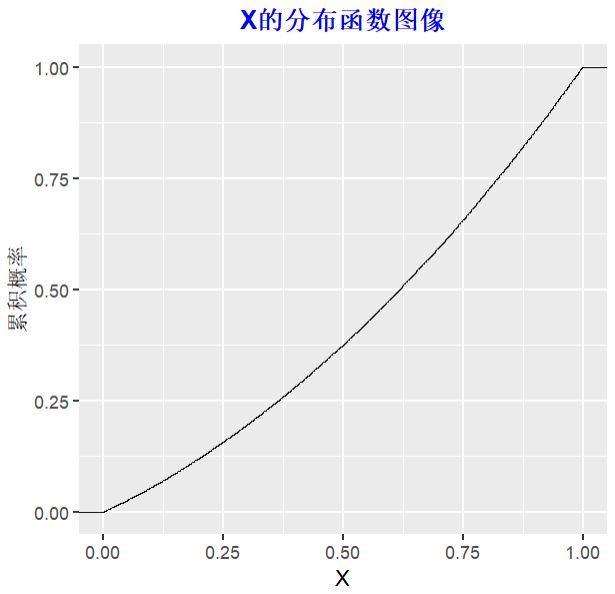
\includegraphics[width = 2.34 in]{gramFile/第三题/分布函数图像.PNG}
      \caption{题3:分布函数}
    \end{minipage}
  }
  \subfigure{
    \begin{minipage}[t]{0.5\linewidth}
      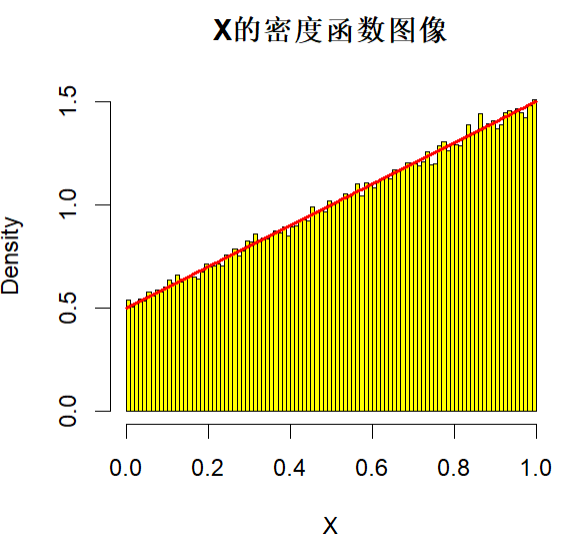
\includegraphics[width = 2.34 in]{gramFile/第三题/概率密度函数图像.PNG}
      \caption{题3:概率密度函数}
    \end{minipage}
  }
\end{figure}

\hspace*{\fill} \\

\noindent
5.5. Give a method for generating a random variable having density function
\begin{equation}
  f(x) =\left\{
  \begin{aligned}
    e^{2x} , \ \ \ -\infty < x < 0 \\
    e^{-2x}, \ \ \ 0 < x < \infty  \\
  \end{aligned}
  \right.
\end{equation}
翻译:给出一种生成具有如上密度函数的随机变量的方法 \\
解:当$x<0$时,
$$
  -\int_{0}^{x}e^{2t}dt = -\frac{1}{2}e^{2t}\bigg|_{0}^{x}
  = \frac{1}{2}(1-e^{2x})
$$
令$x = \frac{1}{2}(1-e^{2y})$,则$y=\ln\sqrt{1-2x}$,则定义域为$x<\frac{1}{2}$ \\
当$x>0$时,
$$
  \int_{0}^{x}e^{-2t}dt = -\frac{1}{2}e^{-2t}\bigg|_{0}^{x}
  = \frac{1}{2}(1-e^{-2x})
$$
令$x = \frac{1}{2}(1-e^{-2y})$,则$y=\ln\sqrt{\frac{1}{1-2x}}$,则定义域为$x<\frac{1}{2}$ \\
代码如下
\lstset{language = R}
\begin{lstlisting}
    n <- 66666
    UR <- runif(n, min = 0, max = 0.5)
    XR <- log(sqrt(1/(1-2*U)))
    UL <- runif(n, min = 0, max = 0.5)
    XL <- log(sqrt(1-2*U))
    X <- append(XR,XL)
    #绘制概率密度图
    hist(X, freq = FALSE, breaks = 100, 
         col = "yellow",
         main = "X的密度函数图像")
    #拟合理论密度曲线
    Y1 <- seq(-5,0,1/100)
    Y2 <- seq(0,5,1/100)
    lines(Y1, exp(2*Y1), col = "red", lwd = 2)
    lines(Y2, exp(-2*Y2), col = "red", lwd = 2)
\end{lstlisting}
第5题运行截图
\begin{figure}[H]
  \centering
  \includegraphics*[height = 7.4cm, width = 8.2cm]{gramFile/第五题/概率密度函数图像.PNG}
  \caption{题5:概率密度函数}
\end{figure}

\hspace*{\fill} \\

\noindent
5.8.Using the result of Exercise 7, give algorithms for generating random variables from
the following distributions. \\
翻译:使用练习7的结论,给出从以下分布生成随机变量的算法 \\
(a) $F(x) = \frac{x+x^3+x^5}{3}, \ \ \ 0 \leq x \leq 1$ \\
解(a):\ \ \ $F(x)=p_{1}F_{1}(x) + p_{2}F_{2}(x) + p_{3}F_{3}(x)$ \\
可以令$p_{1}=p_{2}=p_{3}=\frac{1}{3}$, \ \ \ $F_{1}(x)=x$, \ \ $F_{2}(x)=x^{3}$, \ \ $F_{3}(x)=x^{5}$  \\
(a)题代码如下
\lstset{language = R}
\begin{lstlisting}
    f <- function(n) {
        result <- vector(length = n)
        for(i in 1:n) {
    #每次循环要生成两个随机数,一个随机数用来控制概率
    #另一个随机数用来生成x变量
          U <- runif(2, min = 0, max = 1)
          if(U[1] < 1/3) {
        #有三分之一的概率会生成y=x
            result[i] <- U[2]
          } else if(U[1] < 2/3) {
        #有三分之一的概率会生成y=x^3,那么x就是y^(1/3)
            result[i] <- U[2]^(1/3)
          } else {
        #有三分之一的概率会生成y=x^5,那么x就是y^(1/5)
            result[i] <- U[2]^(1/5)
          }
        }
        #绘制概率密度图
        hist(result, freq = FALSE, breaks = 50,
             col = "yellow", main = "X的密度函数图像")
        Y <- seq(0,1,0.001)
        #拟合理论密度曲线
        lines(Y, (1+3*Y^2+5*Y^4)/3, 
              col = "red", lwd = 2)
    }
    f(66666)
\end{lstlisting}
第8题(a)运行截图
\begin{figure}[H]
  \centering
  \includegraphics*[height = 6.4cm, width = 7.2cm]{gramFile/第八题/(a)题概率密度函数图像.PNG}
  \caption{题8(a):概率密度函数}
\end{figure}

(b) \begin{equation}
  F(x) =\left\{
  \begin{aligned}
     & \frac{1-e^{-2x}+2x}{3} , \ \ \ if \ \ 0 < x < 1                     \\
     & \frac{3-e^{-2x}}{3} , \ \ \ \ \ \ \ \ \ \ \ \ if \ \ 1 < x < \infty \\
  \end{aligned}
  \right.
\end{equation}
解(b):可以令$p_{1}=\frac{2}{3}$, \ \ \ $F_{1}(x) = x$; \ \ \ $p_{2} = \frac{1-e^{-2}}{3}$, \ \ \
$F_{2}(x) = \frac{1-e^{-2x}}{1-e^{-2}}$; \ \ \ $p_{3}=\frac{e^{-2}}{3}$, \ \ \ $F_{3}(x) = 1-e^{-2(x-1)}$ \ \ \
此时$p_{1}+p_{2}+p_{3}=1$, \ \ \ 且保证了$F(1) = p_{1} + p_{2} = \frac{3-e^{-2}}{3}$ ,\ \ \ $F_{1}(0) = 0$, \ \ \ $F_{1}(1) = 1$; \ \ \
$F_{2}(0) = 0$, \ \ \ $F_{2}(1) = 1$; \ \ \ $F_{3}(1) = 0$, \ \ \ $F_{3}(+\infty) = 1$ \\
(b)题代码如下:
\lstset{language = R}
\begin{lstlisting}
    f <- function(n) {
        result <- vector(length = n)
        for(i in 1:n) {
      #每次循环要生成两个随机数,一个随机数用来控制概率
      #另一个随机数用来生成x变量
          U <- runif(2, min = 0, max = 1)
          if(U[1] <= 2/3) {
      #当0<U[1]<p1时,生成服从F1(x)的随机变量
            result[i] <- U[2]
          } else if(U[1] < (3-exp(1)^(-2))/3) {
      #当p1<U[1]<(p1+p2)时,生成服从F2(x)的随机变量
            result[i] <- -0.5*log(1-U[2]*(1-exp(1)^(-2)))
          } else {
      #当(p1+p2)<U[1]<1时,生成服从F3(x)的随机变量
            result[i] <- 1-0.5*log(1-U[2])
          }
        }
        #绘制概率密度图
        hist(result, freq = FALSE, breaks = 100, 
             col = "yellow", main = "X的密度函数图像")
        #拟合理论密度曲线
        Y1 <- seq(0,1,0.001)
        lines(Y1, (2+2*exp(1)^(-2*Y1))/3, 
              col = "red", lwd = 2)
        Y2 <- seq(1,3,0.01)
        lines(Y2, (2*exp(1)^(-2*Y2))/3, 
              col = "red", lwd = 2)
    }
    f(100000)
\end{lstlisting}
第8题(b)运行截图
\begin{figure}[H]
  \centering
  \includegraphics*[height = 6.4cm, width = 7.2cm]{gramFile/第八题/(b)题概率密度函数图像.PNG}
  \caption{题8(b):概率密度函数}
\end{figure}

(c) $F(x) = \Sigma_{i=1}^{n} \alpha_{i}x^{i}, 0 \leq x \leq 1$, \ \ \
where $\alpha_{i} \geq 0$,  \ \ \ $\Sigma_{i=1}^{n} \alpha_{i} = 1$  \\
解(c):此题$\alpha_{i}$可以随机生成, \ $F_{i}(x)$为幂函数,可以瞎令,只需服从指数为正整数且不重复即可  \\
(c)题代码如下
\lstset{language = R}
\begin{lstlisting}
    f <- function(m,n) {
        #随机生成每一个α
        #这里的α是为了保证随机性,方便起见可以自己赋值
    #此处随机生成n个α的原理:
    #首先随机生成n-1个在(0,1)区间的数
        #比如生成了0.49,0.25,0.34,0.08
    #对生成的n-1个数进行排序
        #排序后:0.08,0.25,0.34,0.49
    # 1 = α1 + (α2-α1) + (α3-α2) + (α4-α3) + (1-α4)
    #即生成了:0.08,0.17,0.09,0.15,0.51,加起来刚好是1
        alpha <- vector(length = n)
        R <- runif(n-1, min = 0, max = 1)
        R <- sort(R)
        for(i in 1:length(alpha)) {
          if(i == 1) {
            alpha[i] <- R[i]
          } else if(i == length(alpha)) {
            alpha[i] <- 1-R[i-1]
          } else {
            alpha[i] <- R[i] - R[i-1]
          }
        }
        print(round(alpha,2))
        result <- vector(length = m)
        for(i in 1:m) {
      #每次循环要生成两个随机数,一个随机数用来控制概率
      #另一个随机数用来生成x变量
          U <- runif(2, min = 0, max = 1)
          for(j in 1:n) {
      #循环,看U[1]属于哪一个累积概率区间
            if(U[1] < cumsum(alpha)[j]) {
              result[i] <- (U[2])^(1/(j))
              break
            } 
          }
        }
        #绘制概率密度图
        hist(result, freq = FALSE, breaks = 100, 
             col = "yellow")
        #拟合理论密度曲线
        Y <- seq(0,1,0.00001)
        QX <- vector(length = length(Y))
        for(i in 1:n) {
          QX <-  QX + i * alpha[i] * Y^(i-1)
        }
        lines(Y, QX, col = "red", lwd = 2)
    }
    #多组α取值下的概率密度函数拟合效果
    par(mfrow = c(2,3))
    n <- 300000
    for(i in 2:7) {
      f(n,i)
    }
\end{lstlisting}
第8题(c)运行截图
\begin{figure}[H]
  \centering
  \includegraphics*[height = 3cm, width = 7cm]{gramFile/第八题/(c)题多组α取值结果.PNG}
  \caption{题8(c):多组α取值结果}
\end{figure}
\begin{figure}[H]
  \centering
  \includegraphics*[height = 7.4cm, width = 11.5cm]{gramFile/第八题/(c)题多组α取值下的概率密度函数.PNG}
  \caption{题8(c):多组α取值下的概率密度函数}
\end{figure}

\noindent
(c)题扩充:可以用与(c)题类似的代码模拟出(a)题,代码如下:
\lstset{language = R}
\begin{lstlisting}
    f <- function(m) {
        alpha <- c(1/3,0,1/3,0,1/3)
        print(round(alpha,2))
        result <- vector(length = m)
        for(i in 1:m) {
          U <- runif(2, min = 0, max = 1)
          for(j in 1:5) {
            if(U[1] < cumsum(alpha)[j]) {
              result[i] <- (U[2])^(1/(j))
              break
            } 
          }
        }
        hist(result, freq = FALSE, breaks = 100, 
             col = "yellow", main = "8(a)概率密度图")
        Y <- seq(0,1,0.00001)
        QX <- vector(length = length(Y))
        for(i in 1:5) {
          QX <-  QX + i * alpha[i] * Y^(i-1)
        }
        lines(Y, QX, col = "red", lwd = 2)
      }
      par(mfrow = c(1,1))
      f(100000)
\end{lstlisting}
\begin{figure}[H]
  \centering
  \includegraphics*[height = 6cm, width = 6.8cm]{gramFile/第八题/8(c)类似思路代码模拟8(a).PNG}
  \caption{8(c)类似思路代码模拟8(a)}
\end{figure}

\noindent
5.10. A casually insurance company has 1000 policyholders, each of whom will independently
present a claim in the next month with probability .05. Assuming that the amounts of
the claims made are independent exponential random variables with mean \$800, use
simulation to estimate the probability that the sum of these claims exceeds \$50,000. \\
翻译:一家临时保险公司有1000名投保人,每个投保人将在下个月以0.05的概率独立提出索赔。
假设索赔金额为平均值为800美元的独立指数随机变量,使用模拟来估计这些索赔金额超过
50000美元的概率  \\
解:代码如下
\lstset{language = R}
\begin{lstlisting}
    f <- function(n){
        count <- vector(length = n)
        for(i in 1:n) {
            r <- sample(c(0,1), 1000, replace = TRUE,
                        prob = c(0.95,0.05))
            U <- rexp(10000, 1/800)
            for(j in 1:1000) {
                if(r[j] == 1) {
                  get <- sample(U, 1)
                  count[i] <- count[i] + get
                }
            }
        }
        sum(count > 50000)/n
    }
    f(8888)
\end{lstlisting}
\begin{figure}[H]
  \centering
  \includegraphics*[height = 5cm, width = 7.7cm]{gramFile/第十题/10题运行截图.PNG}
  \caption{第10题模拟结果}
\end{figure}
结论:由模拟结果知,索赔金额超过50000美元的概率为0.1065482

\hspace*{\fill} \\

\noindent
5.14.Let $G$ be a distribution function with density $g$ and suppose, for constants $a < b$,
we want to generate a random variable from the distribution function
$$
  F(x) = \frac{G(x)-G(a)}{G(b)-G(a)}, \ \ \ a \leq x \leq b
$$
(a) If $X$ has distribution $G$, then $F$ is the conditional distribution of $X$ given what information? \\
(b) Show that the rejection method reduces in this case to generating a random variable $X$ having
distribution $G$ and then accepting it if it lies between $a$ and $b$. \\
翻译:设$G$是密度为$g$的分布函数,假设常数$a < b$,我们想从分布函数生成一个随机变量X,且X的分布函数满足上式F(x) \\
(a)如果$X$有分布$G$,那么$F$是给定什么信息的$X$的条件分布? \\
(b)在这种情况下,可简化为用舍选法生成具有分布$G$的随机变量$X$,然后如果它位于$a$和$b$之间,则接受它 \\
解(a):  \\
$F(x)$是由分布函数$G(x)$生成,且给定$F(a)=0,\ \ F(b)=1$的条件分布,且需要满足$G(-\infty)=0, \ \ G(+\infty)=1$ \\
解(b):  \\
"Logistic函数"有一个很好的性质刚好满足题目对$G(x)$的要求,且具有一般性。为方便起见,令$G(x)$为标准"Logistic函数"
$$
  G(x) = \frac{1}{1+e^{-x}}
$$
其满足:\ \ $G(-\infty) = 0$, \ \ $G(+\infty) = 1$,令其导数为$g(x)$
$$
  g(x) = \frac{e^{-x}}{(1+e^{-x})^{2}}
$$
根据题意,用"舍选抽样法"模拟生成具有密度函数为$g(x)$的$X$随机变量,如果随机变量$X$位于$a$与$b$之间,则接受它,
这样就生成了符合条件(其分布函数为$F(x)$)的随机变量$X$  \\
代码如下:
\lstset{language = R}
\begin{lstlisting}
    library(ggplot2)
    Fdistribution <- function(n,a,b){
      k = 0
      z = rep(0,n)
        g <- function(x) {
          gx = 0.5*exp(-x)
          fx =  (exp(-x)) / (1+exp(-x))^2
          cmax <- fx/gx
          return(cmax)
        }
        c <- optimize(g, lower = 0, upper = 100, 
                      maximum = TRUE)$objective
        print(c)
      while(k < n) {
        Df = runif(1)
        x <- -log(Df)   #生成范围在(0,+∞)的随机数
        R = runif(1)
        gx = 0.5*exp(-x)
        fx = (exp(-x)) / (1+exp(-x))^2
        if(c * gx * R <= fx){
          r = runif(1)
    #符合G(x)分布的随机变量的生成,应当正负概率各占一半
    #故当r>0.5时,生成正数,且若该正数位于区间(a,b),则接受它
          if(r > 0.5) {
            if(x > a && x < b) {
              z[k] = x
              k = k + 1
            } 
    #当r<0.5时,生成负数,且若该负数位于区间(a,b),则接受它
          } else {
            if(-x > a && -x < b) {
              z[k] = -x
              k = k + 1
            } 
          }
        }
      }
      return(z) 
    }
    a <- -3
    b <- 2
    resultP <- Fdistribution(188888,-3,2)
    #生成密度函数f(x)
    hist(resultP, prob = TRUE, col = "yellow",
         breaks = 100, main = "X的概率密度函数")
    #拟合理论密度函数曲线
    xx = seq(a,b,1/100) 
    #yy为F(x)的导数,即变量X的密度函数
    yy =   ((1+exp(-a))*(1+exp(-b))*(exp(-xx))) /
           (((1+exp(-xx))^2)*(exp(-a)-exp(-b)))
    lines(xx, yy, col = "red",lwd = 2)
    dataResult <- data.frame(data = resultP)
    #生成分布函数F(x)
    ggplot(dataResult, aes(x = data)) + 
           stat_ecdf(size = 0.1) +      
           labs(title = "X的分布函数图像",
                x = "X",
                y = "累积概率") + 
           theme(plot.title = element_text(
                 color = "blue", 
                 face = "bold", 
                 hjust = 0.5)
                )
\end{lstlisting}
运行结果如下:
\begin{figure}[H]
  \subfigure{
    \begin{minipage}[t]{0.5\linewidth}
      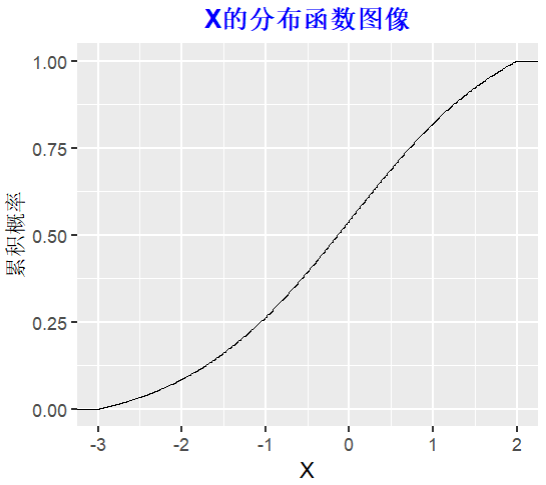
\includegraphics[width = 2.34 in]{gramFile/第十四题/X的分布函数图像.PNG}
      \caption{题14:分布函数}
    \end{minipage}
  }
  \subfigure{
    \begin{minipage}[t]{0.5\linewidth}
      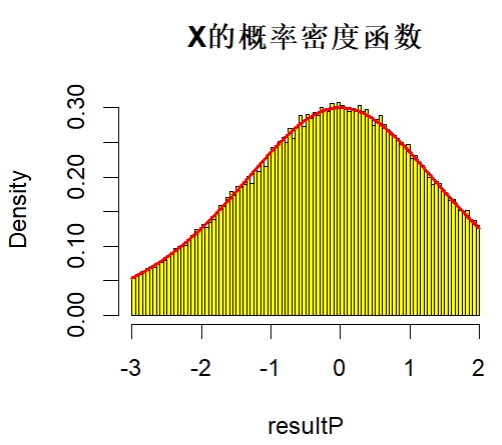
\includegraphics[width = 2.34 in]{gramFile/第十四题/X的概率密度函数.PNG}
      \caption{题14:概率密度函数}
    \end{minipage}
  }
\end{figure}

\noindent
5.19. In Example 5f we simulated a normal random variable by using the rejection technique
with an exponential distribution with rate 1. Show that among all exponential density
functions $g(x) = \lambda e^{-\lambda x}$ the number of iterations needed is minimized when
$\lambda=1$. \\
翻译:
在示例5f中,我们通过使用速率为1的指数分布的舍选抽样法模拟生成了一个正态随机变量。证明在所有的指数密度函数中,
当$\lambda=1$时, \ \ $g(x) = \lambda e^{-\lambda x}$所需的迭代次数最小 \\
解:纯数学证明过程: \\
$$
  f(x) = \frac{2}{\sqrt{2\pi}}e^{\frac{-x^{2}}{2}}  \ \ \ \ 0 < x < \infty \\
$$
$$
  g(x) = \lambda e^{-\lambda x}  \ \ \ \ 0 < x < \infty \\
$$
$$
  C = Max \frac{f(x)}{g(x)} = (\frac{\frac{2}{\sqrt{2\pi}}e^{\frac{-x^{2}}{2}}}{\lambda e^{-\lambda x}})_{max}
  = (\frac{\sqrt{\frac{2}{\pi}} e^{\lambda x - \frac{x^{2}}{2}}}{\lambda})_{max}
$$
\noindent
即转化为求解$F(x) = e^{\lambda x - \frac{x^{2}}{2}}$的最大值,令其导数为$f(x)$,则:
$$
  f(x) = (\lambda - x)e^{\lambda x - \frac{x^{2}}{2}}
$$
故:当$\lambda > x$时,$F(x)$单调递增;当$\lambda < x$时,$F(x)$单调递减;所以在$\lambda = x$时,$F(x)$有最大值,因此:
$$
  C = Max \frac{f(x)}{g(x)}  = \frac{\sqrt{\frac{2}{\pi}} e^{\frac{\lambda ^{2}}{2}}}{\lambda}
$$
现在需要求解当$C$为最小值时,$\lambda$的取值为多少,令$C(\lambda) = \frac{e^{\frac{\lambda ^{2}}{2}}}{\lambda}$ \\
则其导数$c(\lambda)$为:
$$
  c(\lambda) = \frac{(\lambda^{2}-1)e^{\frac{\lambda^{2}}{2}}}{\lambda^{2}}
$$
故:当$\lambda > 1$时,$C(\lambda)$单调递增;当当$0 < \lambda < 1$时,$C(\lambda)$单调递减;所以当$\lambda = 1$时,C有最小值。
以下用计算机程序模拟:
\lstset{language = R}
\begin{lstlisting}
    n <- 120
    c <- data.frame(lambda = rep(0,n),
                    cMax = rep(0,n))
    Df <- seq(0,3,0.025)
    f <- function(lambda) {
      g <- function(x) {
        gx = lambda*exp(-lambda*x)
        fx = (2/pi)^(1/2)*exp(-1/2*x^2)
        cmax <- fx/gx
      }
      #求解在每一个λ水平下的C值(迭代次数)
      result <- optimize(g, lower = 0, upper = 10,
                         maximum = TRUE)$objective
      answerLambda <- optimize(g, lower = 0,
                upper = 10, maximum = TRUE)$maximum
      re <- list(cMax = result, 
                 aL = round(answerLambda,3))
      return(re)
    }
    for(i in 1:n) {
        c[i,1] <- f(Df[i+1])$aL
        c[i,2] <- f(Df[i+1])$cMax
    }
    plot(x = c$lambda, y = c$cMax, col = "purple")
    #找到迭代次数最小的所在行
    row <- which.min(c$cMax)
    c[row,]
\end{lstlisting}
运行结果如下:
\begin{figure}[H]
  \centering
  \includegraphics*[height = 4.5cm, width = 5.7cm]{gramFile/第十九题/不同λ取值下的迭代次数分布.PNG}
  \caption{19题:不同λ取值下的迭代次数分布}
\end{figure}
\noindent
由上图知,迭代次数随着$\lambda$取值的增加,先是单调递减,然后是单调递增
\begin{figure}[H]
  \centering
  \includegraphics*[height = 1.28cm, width = 4cm]{gramFile/第十九题/迭代次数最小时的λ取值.PNG}
  \caption{19题:迭代次数最小时的λ取值}
\end{figure}
\noindent
由上图结果知:迭代次数在$\lambda=1$时取到最小值,且最小迭代次数为1.315489

\hspace*{\fill} \\

\noindent
5.20. Write a program that generates normal random variables by the method of Example 5f. \\
翻译:用5f的方法编写一个程序生成服从正态分布的随机变量 \\
解:代码如下
\lstset{language = R}
\begin{lstlisting}
    #n为模拟次数;mu为均值;sigma为标准差
    normalDis <- function(n, mu, sigma){
        k = 0
        z = rep(0,n)
          g <- function(x) {
            gx = exp(-x)
            fx = (1 / ((sqrt(2*pi)) * sigma)) *
                 (exp( - (x-mu)^2 / (2*sigma^2)))
            cmax <- fx/gx
          }
          c <- optimize(g, lower = -10, upper = 10,
                        maximum = TRUE)$objective
        while(k < n) {
          Df = runif(1)
          #生成范围在(mu,+∞)的随机数
          x = -log(Df) + mu  
          R = runif(1)
          gx = exp(-x)
          fx = (1 / ((sqrt(2*pi)) * sigma)) *
               (exp( - (x-mu)^2 / (2*sigma^2)))
          if(c * gx * R <= fx){
            r = runif(1)
    #生成的随机数应当有一半的概率大于mu,一半的概率小于mu
    #故当r<0.5时,生成大于mu的随机数(上面生成的x刚好大于mu)
            if(r < 0.5) {  
              z[k] = x
            } else {
    #当r>0.5时,生成小于mu的随机数(-x+2mu刚好符合这个条件)
    #因为-x属于(-∞,-mu)区间,则-x+2mu属于(-∞,mu)区间
              z[k] = -x + 2*mu
            }
            k = k + 1
          }
        }
        return(z) 
      }
      #不同均值和方差的正态分布模拟
      #由于模拟次数太大,且在舍选抽样法中对于方差过大的
      #正态分布模拟效果较低,故只选取方差较小的正态分布
      #进行模拟,否则容易死机
      par(mfrow = c(3,3))
      #变量"i"控制均值;变量"j"控制标准差
      for(i in 1:3) {
        for(j in 1:3) {
          mu <- i
          sigma <- j
          #生成正态分布的密度函数
          hist(normalDis(66666, mu, sigma), 
               prob = TRUE, col = "yellow", 
               breaks = 100, main = "正态分布图")
          #拟合理论密度函数曲线
          xx = seq(-20,20,1/100) 
          yy = (1 / ((sqrt(2*pi)) * sigma)) *
               (exp ( - (xx-mu)^2 / (2*sigma^2) ) )
          lines(xx, yy, col = "red",lwd = 2)
        }
      }
\end{lstlisting}
\begin{figure}[H]
  \centering
  \includegraphics*[height = 10cm, width = 11.5cm]{gramFile/第二十题/九组不同均值和标准差取值下的模拟结果.PNG}
  \caption{20题:九组不同均值和标准差取值下的模拟结果}
\end{figure}
\noindent
注意:从左到右,标准差依次增大;从上到下,均值依次增大

\hspace*{\fill} \\

\noindent
5.22. Write a program that generates the first $T$ time units of a Poisson process having rate $\lambda$. \\
翻译:编写一个程序,生成具有速率为$\lambda$的前$T$个时间单位的泊松过程 \\
解:代码如下:
\lstset{language = R}
\begin{lstlisting}
    f <- function(lambda, T) {
        g <- function(lambda, T) {
          #S数组用来存储每次事件发生的时间
          S <- vector(length = 10*lambda*T)
          t = 0
          #C为事件发生次数
          C = 0
          for(i in 1:length(S)) {
            Df = runif(1)
            x = -log(Df)  #生成范围在(0,+∞)的随机数
            t = t+x/lambda
            #若时间累加大于既定时间,则退出循环
            if(t > T) {
              break
            } 
            C = C+1
            S[C] = t
          }
          re <- list(count = C)
          return(re)
        }
        n <- 66666
        resultCount <- vector(length = n)
        for(i in 1:n) {
          re <- g(lambda, T)
          resultCount[i] <- re$count 
        }
        print(mean(resultCount))
        #生成次数分布图
        hist(resultCount, freq = FALSE,  
             col = "yellow", main = "次数分布图",
             xlab = "次数", ylab = "频率",
             breaks = 30)
    }
    par(mfrow = c(2,2))
    #模拟四组结果
    f(3, 6)
    f(4, 5)
    f(10,3)
    f(5, 8)
\end{lstlisting}
运行结果如下:
\begin{figure}[H]
  \centering
  \includegraphics*[height = 8.8cm, width = 11.5cm]{gramFile/第二十二题/不同λ和T取值下的泊松过程.PNG}
  \caption{22题:四组不同λ和T取值下的泊松过程}
\end{figure}
\begin{figure}[H]
  \centering
  \includegraphics*[height = 2.8cm, width = 2cm]{gramFile/第二十二题/四组不同λ和T取值的齐次泊松过程模拟.PNG}
  \caption{22题:四组不同λ和T取值的齐次泊松过程模拟}
\end{figure}

\noindent
5.23. To complete a job a worker must go through $k$ stages in sequence. The time to complete stage $i$ is an
exponential random variable with rate $\lambda_{i}$, $i = 1,...,k$. However, after
completing stage $i$ the worker will only go to the next stage with probability $\alpha_{i}$, $i = 1,...,k-1$.
That is, after completing stage $i$ the worker will stop working with probablity $1-\alpha_{i}$, If we let $X$
denote the amount of time that the worker spends on the job, the $X$ is called a Coxian random variable.
Write an algorithm for generating such a random variable. \\
翻译:
要完成一项工作,工人必须依次经历$k$个阶段。完成阶段$i$的时间是一个指数随机变量,速率$\lambda_{i}$, $i = 1,...,k$。然而,
在完成第$i$阶段后,工人将仅以概率$\alpha_{i}$, $i = 1,...,k-1$进入下一阶段。也就是说,在完成第一阶段后,员工将以概率$1-\alpha
  _{i}$停止工作。如果我们让$X$表示工人在工作上花费的时间量,则$X$被称为$Coxian$随机变量。编写一个生成这样一个随机变量的算法. \\
解:代码如下:
\lstset{language = R}
\begin{lstlisting}
  #参数k为工作阶段数,参数n为工人人数
  g <- function(k,n) {  
    #随机生成k个λ:
    lambda <- vector(length = k)
    for(i in 1:k) {
      lambda[i] <- runif(1, min = 0, max = 10)
    }
    print("λ的值为:")
    print(lambda)
    #随机生成k-1个α:
    alpha <- vector(length = k-1)
    for(i in 1:k-1) {
      alpha[i] <- runif(1, min = 0, max = 1) 
    }
    print("α的值为:")
    print(alpha)
    #生成m <= k轮服从指数分布的随机变量
    f <- function(k){
        T <- vector(length = k)
        #每个工人都会参与第一阶段的工作
        T[1] <- rexp(1, rate = lambda[1])
        for(i in 2:k) {
          #判断下一阶段是否工作
          R <- sample(c(0,1), 1, 
               prob = c(1-alpha[i-1], alpha[i-1]))
          #不工作直接退出
          if(R == 0) {
            break
          } 
          #继续工作的把工时加上
          T[i] <- rexp(1, rate = lambda[i])
        }
        return(round(sum(T),3))
    }
    #重复n次实验(相当于n个工人样本)
    result <- vector(length = n)
    for(j in 1:n) {
      result[j] <- f(k)
    }
    hist(result, main = "工人工作时间分布图",
         xlab = "工作时间", ylab = "频率",
         col = "green", freq = FALSE, breaks = 50)
    print("在该组λ和α取值情况下,工人的平均工作时间如下")
    print(mean(result))
    #计算理论工作时长
    print("在该组λ和α取值情况下,工人的理论工作时间如下")
    sum <- 1/lambda[1]
    for(i in 2:k) {
      sum <-  sum + cumprod(alpha)[i-1] / lambda[i]
    }
    print(sum)
  }
  #重复6次模拟实验
  par(mfrow = c(3,2))
  for(k in 2:7) {
    print("---------------------------------")
    g(k,100000)
  }
\end{lstlisting}
运行结果如下:
\begin{figure}[H]
  \centering
  \includegraphics*[height = 5.8cm, width = 7.5cm]{gramFile/第二十三题/前两组不同λ和α取值下的工人工作时间模拟结果.PNG}
  \caption{23题:前两组不同λ和α取值下的工人工作时间模拟结果}
\end{figure}
\begin{figure}[H]
  \centering
  \includegraphics*[height = 5.8cm, width = 8.5cm]{gramFile/第二十三题/中间两组不同λ和α取值下的工人工作时间模拟结果.PNG}
  \caption{23题:中间两组不同λ和α取值下的工人工作时间模拟结果}
\end{figure}
\begin{figure}[H]
  \centering
  \includegraphics*[height = 5.8cm, width = 10.5cm]{gramFile/第二十三题/后两组不同λ和α取值下的工人工作时间模拟结果.PNG}
  \caption{23题:后两组不同λ和α取值下的工人工作时间模拟结果}
\end{figure}
\begin{figure}[H]
  \centering
  \includegraphics*[height = 10cm, width = 11cm]{gramFile/第二十三题/6组不同λ和α取值下的工人工作时间分布图.PNG}
  \caption{23题:6组不同λ和α取值下的工人工作时间分布图}
\end{figure}

\noindent
5.24.Buses arrive at a sporting event according to a Poisson process with rate 5 per hour. Each bus is equally
likely to contain either 20,21,...,40 fans, with the numbers in the different buses being independent.
Write an algorithm to simulate arrival of fans to the event by time $t = 1$.  \\
翻译:
公交车按照泊松过程到达体育赛事,速度为每小时5辆。每个总线都可能包含20,21,...,40个风扇,不同总线中的数字是独立的。编写一个
算法,模拟"粉丝在时间$t=1$之前到达"这个事件. \\
解:代码如下:
\lstset{language = R}
\begin{lstlisting}
  f <- function(n) {
    fansN <- vector(length = n)
    for(i in 1:n) {
      amount <- rpois(1, lambda = 5)
      fansCount <- vector(length = amount)
      for(j in 1:amount) {
        fansCount[j] <- sample(20:40, 1)
      }
      fansN[i] <- sum(fansCount)
    }
    print(mean(fansN))
  }
  f(16666)
\end{lstlisting}
运行结果如下:
\begin{figure}[H]
  \centering
  \includegraphics*[height = 4.5cm, width = 7cm]{gramFile/第二十四题/模拟事件---粉丝在T=1之前到达.PNG}
  \caption{24题:模拟事件---粉丝在T=1之前到达}
\end{figure}

\noindent
5.25.
(a) Write a program that uses the thinning algorithm to generate the first 10 time units of a nonhomogeneous
Poisson process with intensity function.
$$
  \lambda(t)=3+\frac{4}{t+1}
$$
(b) Give a way to improve upon the thinning algorithm for this example.  \\
翻译:
(a)编写一个程序,使用"瘦身"算法生成具有如上强度函数的前10个时间单位的非齐次泊松过程 \\
(b)给出一种改进本例"瘦身"算法的方法 \\
解:(a)题代码如下:
\lstset{language = R}
\begin{lstlisting}
  fa <- function(T) {
    h <- function(t) {
      return(3+4/(t+1))
    } 
    #求解最大的λ值
    hMax <- optimize(h, lower = 0, 
            upper = T, maximum = TRUE)$objective
    g <- function(T) {
      #S数组用来存储每次事件发生的时间
      S <- vector(length = 100)
      t = 0
      #C为事件发生次数
      C = 0
      for(i in 1:100000) {
        Df = runif(1)
        x = -log(Df)  #生成范围在(0,+∞)的随机数
        t = t+x/hMax
        #若时间累加大于既定时间,则退出循环 
        if(t > T) {
          break
        } 
        R <- runif(1)
        if(R <= h(t)/hMax){
          C = C+1
          S[C] = t
        }      
      } 
      #循环结束后返回事件发生次数
      re <- list(count = C)
      return(re)
    }
    n <- 10000
    resultCount <- vector(length = n)
    for(i in 1:n) {
      re <- g(T)
      resultCount[i] <- re$count 
    }
    print(mean(resultCount))
    #输出非齐次泊松过程的次数分布图
    hist(resultCount, freq = FALSE, 
         col = "yellow", main = "次数分布图",
         xlab = "次数",  ylab = "频率", 
         breaks = 30)
  }
  par(mfrow = c(1,1))
  #计算运行时间
  ptmf <- proc.time()
  fa(10)
  print(proc.time() - ptmf)
\end{lstlisting}
(a)题运行结果如下:
\begin{figure}[H]
  \centering
  \includegraphics*[height = 2.3cm, width = 4.8cm]{gramFile/第二十五题/(a)题---瘦身法模拟非齐次泊松过程---运行结果与运行时间.PNG}
  \caption{25(a):瘦身法模拟非齐次泊松过程---运行结果与运行时间}
\end{figure}
\begin{figure}[H]
  \centering
  \includegraphics*[height = 5cm, width = 7cm]{gramFile/第二十五题/(a)题---瘦身法模拟非齐次泊松过程---次数分布图.PNG}
  \caption{25(a):瘦身法模拟非齐次泊松过程---次数分布图}
\end{figure}

\noindent
解:(b)题代码如下:
\lstset{language = R}
\begin{lstlisting}
  #参数T为时间,参数k为分段区间个数
  fb <- function(T,k) {
    h <- function(t) {
      return(3+4/(t+1))
    }
    #变量r用来存储每个区间的右边界
    #其实为保证随机性,区间分段应是任意的,但这里采用均匀分段
    r <- seq(0,T,len=k+1)
    #求解每个分段区间内的λ的最大值
    hMax <- vector(length = k)
    for(i in 1:k) {
      hMax[i] <- optimize(h, lower = r[i],
              upper = r[i+1],
              maximum = TRUE)$objective
    }
    r <- r[2:length(r)]
    g <- function(T) {
      #S数组用来存储每次事件发生的时间
      S <- vector(length = 10000)
      t = 0
      #C为事件发生次数
      C = 0
      #变量J用来记录当前事件发生在哪一个区间内
      J = 1
      for(i in 1:length(S)) {
        Df = runif(1)
        x = -log(Df)/hMax[J] 
        #当累加时间大于某分区间的右边界时,J应当+1
        while(t+x > r[J] && J!=k+1) {
          x = (x-r[J]+t) * hMax[J]  / hMax[J+1] 
          t = r[J]
          J = J + 1
        }
        #如果区间越过规定截止时间,则退出整个循环
        if(J==k+1) {
          break
        } 
        t = t+x
        R <- runif(1)
        if(R <= h(t)/hMax[J]) {
          C = C+1
          S[C] = t
        }
      }
      #整个循环结束后返回事件发生次数
      re <- list(count = C)
      return(re)
    }
    n <- 10000
    resultCount <- vector(length = n)
    for(i in 1:n) {
      re <- g(T)
      resultCount[i] <- re$count 
    }
    print(mean(resultCount))
    #输出非齐次泊松过程的次数分布图
    hist(resultCount, freq = FALSE,
         col = "yellow", main = "次数分布图",
         xlab = "次数",  ylab = "频率", 
         breaks = 30)
  }
  ptmf <- proc.time()
  fb(10,25)
  print(proc.time() - ptmf)
\end{lstlisting}
(b)题运行结果如下:
\begin{figure}[H]
  \centering
  \includegraphics*[height = 2.3cm, width = 4.8cm]{gramFile/第二十五题/(b)题---分段瘦身法模拟非齐次泊松过程---运行结果与运行时间.PNG}
  \caption{25(b):分段瘦身法模拟非齐次泊松过程---运行结果与运行时间}
\end{figure}
\begin{figure}[H]
  \centering
  \includegraphics*[height = 5cm, width = 7cm]{gramFile/第二十五题/(b)题---分段瘦身法模拟非齐次泊松过程---次数分布图.PNG}
  \caption{25(b):分段瘦身法模拟非齐次泊松过程---次数分布图}
\end{figure}
\noindent
注意:两种算法的模拟次数必须一致,否则没有比较意义 \\
且从统计的角度看,各方法只模拟一次就说哪个算法效率高是不太靠谱的,因此可以多模拟几次,此处就不展示了

\noindent
5.26.Give an efficient algorithm to generate the first 10 times units of a nonhomogeneous Poisson process having intensity function \\
\begin{equation}
  \lambda(t) =\left\{
  \begin{aligned}
     & \frac{t}{5}, \ \ \ \ \ \ \ \ \ \ \ \ \ \ \ \ \ \ \ \ 0 < t < 5 \\
     & 1+5(t-5), \ \ 5 < t < 10                                       \\
  \end{aligned}
  \right.
\end{equation}
翻译:
给出一种有效的算法来生成具有如上强度函数的前10个单位的非齐次泊松过程 \\
\noindent
解:26题和25题思路一模一样,分别用瘦身法和分段瘦身法模拟,并比较哪一种算法效率更高 \\
(法一)瘦身法代码如下:
\lstset{language = R}
\begin{lstlisting}
  fa <- function(T) {
    h <- function(t) {
      if(t < 5) {
        return(t/5)
      } else if(t < 10){
        return(1+5*(t-5))
      } 
    }
    #求解最大的λ值
    hMax <- optimize(h, lower = 0,
            upper = T, maximum = TRUE)$objective
    g <- function(T) {
      S <- vector(length = 100)
      t = 0
      C = 0
      for(i in 1:6666666) {
        Df = runif(1)
        x = -log(Df)  #生成范围在(0,+∞)的随机数
        t = t+x/hMax 
        if(t > T) {
          break
        } 
        R <- runif(1)
        if(R <= h(t)/hMax){
          C = C+1
          S[C] = t
        }      
      } 
      re <- list(count = C)
      return(re)
    }
    n <- 10000
    resultCount <- vector(length = n)
    for(i in 1:n) {
      re <- g(T)
      resultCount[i] <- re$count 
    }
    print(mean(resultCount))
    #输出非齐次泊松过程的次数分布图
    hist(resultCount, freq = FALSE,
         col = "yellow", main = "次数分布图",
         xlab = "次数",  ylab = "频率",
         breaks = 30)
  }
  ptmf <- proc.time()
  fa(10)
  print(proc.time() - ptmf)
\end{lstlisting}

\noindent
(法二)分段瘦身法代码如下:
\lstset{language = R}
\begin{lstlisting}
  #参数T为时间,参数k为分段区间个数
  fb <- function(T,k) {
    h <- function(t) {
      if(t < 5) {
        return(t/5)
      } else if(t < 10){
        return(1+5*(t-5))
      }
    }
    r <- seq(0,T,len=k+1)
    #求解每个分段区间内的λ的最大值
    hMax <- vector(length = k)
    for(i in 1:k) {
      hMax[i] <- optimize(h, lower = r[i],
            upper = r[i+1], maximum = TRUE)$objective
    }
    r <- r[2:length(r)]
    g <- function(T) {
      S <- vector(length = 10000)
      t = 0
      C = 0
      J = 1
      for(i in 1:length(S)) {
        Df = runif(1)
        x = -log(Df)/hMax[J] 
        while(t+x > r[J] && J!=k+1) {
          x = (x-r[J]+t) * hMax[J]  / hMax[J+1] 
          t = r[J]
          J = J + 1
        }
        if(J==k+1) {
          break
        } 
        t = t+x
        R <- runif(1)
        if(R <= h(t)/hMax[J]) {
          C = C+1
          S[C] = t
        }
      }
      re <- list(count = C)
      return(re)
    }
    n <- 10000
    resultCount <- vector(length = n)
    for(i in 1:n) {
      re <- g(T)
      resultCount[i] <- re$count 
    }
    print(mean(resultCount))
    #输出非齐次泊松过程的次数分布图
    hist(resultCount, freq = FALSE,
         col = "yellow", main = "次数分布图",
         xlab = "次数",  ylab = "频率",
         breaks = 30)
  }
  ptmf <- proc.time()
  fb(10,30)
  print(proc.time() - ptmf)
\end{lstlisting}
\noindent
同样的,可以多模拟几次增强说服力,这里就不再展示了\\
运行结果如下:
\begin{figure}[H]
  \subfigure{
    \begin{minipage}[t]{0.5\linewidth}
      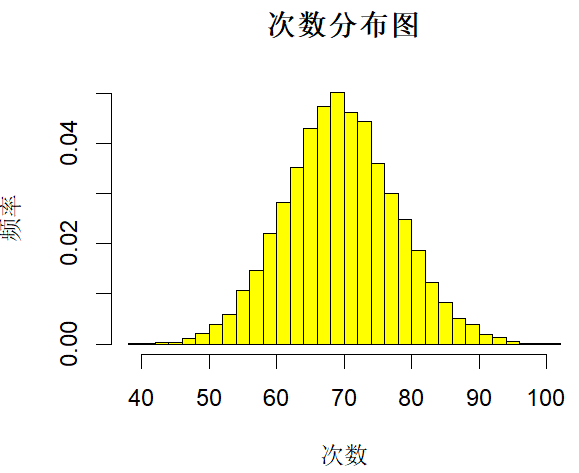
\includegraphics[width = 2.44 in]{gramFile/第二十六题/瘦身法模拟---次数分布图.PNG}
      \caption{题26:瘦身法次数分布图}
    \end{minipage}
  }
  \subfigure{
    \begin{minipage}[t]{0.5\linewidth}
      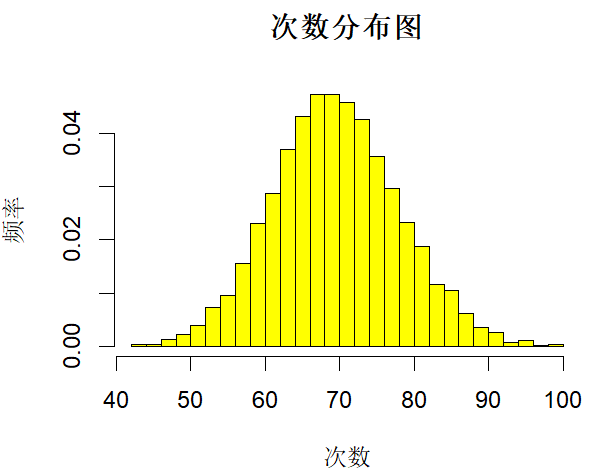
\includegraphics[width = 2.44 in]{gramFile/第二十六题/分段瘦身法模拟---次数分布图.PNG}
      \caption{题26:分段瘦身法次数分布图}
    \end{minipage}
  }
\end{figure}
\begin{figure}[H]
  \subfigure{
    \begin{minipage}[t]{0.5\linewidth}
      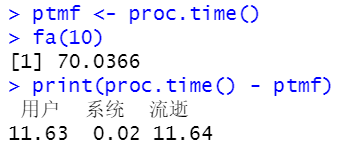
\includegraphics[width = 2.34 in]{gramFile/第二十六题/瘦身法模拟---运行时间.PNG}
      \caption{题26:瘦身法运行时间}
    \end{minipage}
  }
  \subfigure{
    \begin{minipage}[t]{0.5\linewidth}
      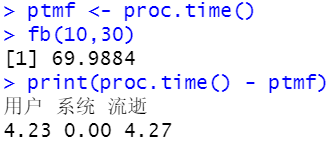
\includegraphics[width = 2.34 in]{gramFile/第二十六题/分段瘦身法模拟---运行时间.PNG}
      \caption{题26:分段瘦身法运行时间}
    \end{minipage}
  }
\end{figure}
\noindent
结论:显然,分段瘦身法模型效率更高 \\
注意:两种算法的模拟次数必须一致,否则没有比较意义

\end{document}